\documentclass{article}

\newcommand{\plotsize}{0.23}

\usepackage{graphicx}
\graphicspath{{./images/}}

\usepackage{float}
\usepackage{hyperref}
\usepackage{listings}
\lstset{
	basicstyle=\ttfamily,
	columns=fullflexible,
	frame=single,
	breaklines=true,
	postbreak=\mbox{\textcolor{black}{$\hookrightarrow$}\space},
}

% margins of 1 inch:
\setlength{\topmargin}{-.5in}
\setlength{\textheight}{9.5in}
\setlength{\oddsidemargin}{0in}
\setlength{\textwidth}{6.5in}

\usepackage{hyperref}
\hypersetup{
    colorlinks=true,
    linkcolor=blue,
    filecolor=magenta,      
    urlcolor=cyan,
    pdftitle={Overleaf Example},
    pdfpagemode=FullScreen,
    }

\begin{document}


% Relevant links and notes.
%
%	https://en.wikipedia.org/wiki/Deadlock
%	https://en.wikipedia.org/wiki/Discrete-event_simulation
%	http://sst-simulator.org/
%
%

    % https://stackoverflow.com/a/3408428/1164295
    %\begin{minipage}[h]{\textwidth}
        \title{2022 Future Computing Summer Internship Project:\\Modeling Deadlock in a Discrete-Event Simulator to Find Metrics to Measure its Existence in a Simulation}
        \author{Nicholas Schantz\thanks{nschantz3@gatech.edu}}
        \date{\today}
            \maketitle
        \begin{abstract}
            \href{https://en.wikipedia.org/wiki/Deadlock}{Deadlock} is an issue that can occur in distributed systems in which multiple nodes connected in a cycle cannot proceed with any action because they are waiting for each other to take action as well. This research addresses the question as to whether metrics exist to determine if this problem has occurred in a distributed system simulation. These metrics are useful for system architects to monitor distributed system simulations and catch when deadlock occurs, and they can fix any issues before the system is put into production. The \href{https://en.wikipedia.org/wiki/Discrete-event_simulation}{discrete-event simulator} (DES) framework named \href{http://sst-simulator.org/}{Structural Simulation Toolkit} (SST) is used to simulate this activity and find a metric. An SST model is created of a network of nodes in a \href{https://en.wikipedia.org/wiki/Ring_network}{ring topology} that pass messages in one direction to a connected node's queue. Messages are generated by nodes and sent out which result in deadlock if the nodes' queues fill up before the messages can reach their destination. Metrics to detect deadlock include measuring for a cycle of blocked nodes, how often a node changes from executing to idling, how many times the nodes have requested a resource while idle, and how long the nodes are idle. Utilizing these metrics, detection for system-scale deadlock was found. A global node that logs all other nodes' data can be used to determine if there is a high number of requests for nodes' queues even if all nodes are in an idle state. Nodes can also self detect for deadlock by sending around a probe that will measure if a cycle of blocked nodes exist in the simulation. Further progress needs to be made regarding if metrics exist for detecting if a component-scale deadlock exists in a simulation.
        \end{abstract}
    %\end{minipage}

\ \\
% see https://en.wikipedia.org/wiki/George_H._Heilmeier#Heilmeier's_Catechism

%\maketitle

\section{Project Description} % what problem is being addressed? 

The challenge addressed by this work is to map the distributed systems problem deadlock to a discrete-event simulator. \href{https://www.sandia.gov/}{Sandia National Laboratories'} Structural Simulation Toolkit is a discrete-event simulator framework which is used to simulate the problem. Simulation output is collected to help identify mathematical or logical conditions that can cause this problem. This information is used to develop metrics to identify that the problem has occurred in simulated distributed systems.

\section{Motivation} % Why does this work matter? Who cares? If you're successful, what difference does it make?
Identifying the metrics to detect deadlock will be vital for developing distributed systems that avoid this problem from occurring. System architects may be unaware of this problem or may not know that a deadlock can occur in their distributed system simulation. The metrics found in this research can help them catch this problem when they occur in simulation so that the problem can be prevented when the system is put into production.

A second goal of this work is to develop examples and documentation of SST simulations that new users can utilize. Currently, SST is primarily used for \href{https://en.wikipedia.org/wiki/High-performance_computing}{High-Performance Computing} (HPC) simulations and the majority of the SST examples revolve around modeling HPC systems. However, the SST framework utilizes a powerful discrete-event simulator that can model more than just HPC systems. The models and documentation created for this project show off the discrete-event simulations not relating to HPC systems.

\section{Prior work} % what does this build on?

Chandy and Mishra \cite{1983_Chandy} researched and developed a distributed deadlock detection algorithm that measures for cycles of blocked processes that depend on each other. This work inspired the deadlock detection metric for the first SST model explained in section \nameref{sst_model}.

\section{Running the Model}

The software developed for this challenge was run on one laptop running an Ubuntu-Based Linux operating system. The software is available at \href{https://github.com/lpsmodsim/2022HPCSummer-CongestiveCollapse}{https://github.com/lpsmodsim/2022HPCSummer-CongestiveCollapse}.\newline

\noindent Assuming the user is on a system running a Ubuntu-Based Linux Distro. To run the software:\newline

\noindent Prerequisites: 

\begin{verbatim}
	sudo apt install singularity black mypi
	git clone https://github.com/tactcomplabs/sst-containers.git
\end{verbatim}

\noindent Follow the instructions in the git repo to build the container "sstpackage-11.1.0-ubuntu-20.04.sif".

\begin{verbatim}
	cp sst-containers/singularity/sstpackage-11.1.0-ubuntu-20.04.sif /usr/local/bin/
	git clone https://github.com/lpsmodsim/2022HPCSummer-SST.git
	sudo . /2022HPCSummer-SST/additions.def.sh
\end{verbatim}

\noindent Obtaining and running the model:

\begin{verbatim}
	git clone https://github.com/lpsmodsim/2022HPCSummer-Deadlock
	cd 2022HPCSummer-Deadlock/deadlock
	make
\end{verbatim}

\noindent To re-run the software:

\begin{verbatim}
	make clean
	make
\end{verbatim}

\noindent Expected output:

\begin{lstlisting}[language=bash, frame=none]
mkdir -p .build
singularity exec /usr/local/bin/additions.sif g++ -std=c++1y -D__STDC_FORMAT_MACROS -fPIC -DHAVE_CONFIG_H -I/opt/SST/11.1.0/include -MMD -c node.cc -o .build/node.o
singularity exec /usr/local/bin/additions.sif g++ -std=c++1y -D__STDC_FORMAT_MACROS -fPIC -DHAVE_CONFIG_H -I/opt/SST/11.1.0/include -shared -fno-common -Wl,-undefined -Wl,dynamic_lookup -o libdeadlock.so .build/node.o
singularity exec /usr/local/bin/additions.sif sst-register deadlock deadlock_LIBDIR=/home/{USER}/sst-work/2022HPCSummer-Deadlock/deadlock
singularity exec /usr/local/bin/additions.sif black tests/*.py
singularity exec /usr/local/bin/additions.sif mypy tests/*.py
Success: no issues found in 2 source files
singularity exec /usr/local/bin/additions.sif sst tests/deadlockrand.py
(Simulation console output)
\end{lstlisting}

\noindent The simulation can be modified by editing the python driver file, which is located at:

\begin{verbatim}
	2022HPCSummer-Deadlock/tests/deadlock.py
\end{verbatim}

\section{The Model}
\label{sst_model}
The models created for the deadlock problem were a network of \textit{n} nodes in a ring topology passing messages along the ring in one direction. The model was built with the conditions for deadlock in mind. The conditions are the following\cite[p. 70]{1971_Coffman}:

\begin{itemize}
	\label{list:conditions}
	\item Mutual Exclusion - Process has exclusive access to the resource it is holding.
	\item Wait For - A process will hold on to a resource while its waiting for a new one.
	\item No Preemption - A process cannot remove a resource from another process.
	\item Circular Wait - The processes which are holding and requesting resources form a cycle. \newline
\end{itemize}

These conditions can be related to the SST model by the following:

\begin{itemize}
	\item Mutual Exclusion - Each node has exclusive access to the next node's queue.
	\item Wait For - Each node waits and makes requests to send messages to the next node's finite queue.
	\item No Preemption - A node cannot force the next node to send messages out and free up its queue.
	\item Circular Wait - The nodes form a cyclic connection.
\end{itemize}

Two models with slight differences were created to demonstrate deadlock and how to detect the problem. The first model only consist of nodes in a ring topology, while the the second model introduces a node that collects logging data from all the nodes in the ring topology. The second model gives more freedom on how we can use information shared between all nodes to form metrics to detect deadlock in the simulation.

\begin{figure}[H]
	\includegraphics[scale=0.5]{deadlock-fix}\newline
	\centering
	\caption{Example of first model with three nodes.}
	\centering
\end{figure}

\begin{figure}[H]
	\includegraphics[scale=0.5]{deadlocktest}\newline
	\centering
	\caption{Example of second model with three nodes connected to one central logging node.}
	\centering
\end{figure}

An issue with these models is that the conditions for deadlock are baked into the models to force deadlock to occur. To improve the models, the conditions should be variable to get a more generalized system to collect metrics as to when deadlock exists in a simulation. This model is one specific example of deadlock in which measurements can be collected to detect why deadlock is occurring in this model, but does not determine for all cases if deadlock has occurred. For example, in a communication model of deadlock where messages are passed along, nodes' send rates can cause deadlocks to occur if all nodes' queues are filled up before messages reach their destination. However, send rate could be irrelevant for a deadlock occurring between processes grabbing resources. 

\section{Result} % conclusion/summary

The results found so far is that system-scale deadlock can be detected in a simulation. The metrics to detect for deadlock differ in the two models.

In the first model, a global logging node does not exist so a node can only initially detect that it is in a blocked state but does not know if the system is in deadlock. When a node detects that it is in a blocked state, an algorithm is used for it to detect if a system-scale deadlock has occurred. The algorithm is used to measure a cycle of blocked processes in the system and is based on the resource model deadlock detection found in \cite[p. 149]{1983_Chandy}. The algorithm utilizes messages called ``probe'' which are sent and read by other nodes immediately instead of being stored in a queue. When a node cannot access the next node's queue, it is blocked and will send out a probe to the next node. The probe will keep track of the originator and whether or not the current holder is also blocked from sending messages. When the probe is received by a node, it will pass the probe along if it is in a blocked state, otherwise it will drop the probe. If a node receives a probe that originated from itself, then a ring of blocked nodes has been measured which means that the ring of nodes are deadlocked. In this model, this means that a system-scale deadlock has occurred since the model is made of a ring of nodes.

In the second model, a global logging node does exist which can keep track of all other nodes' states and determine if they are all in a blocked state. The global logging node will track what nodes are executing or idle, how many times they have requested to send a message to a connected nodes queue while idle, and how many times they have changed states during the simulation. From plotted data, deadlock will occur when all nodes idle time linearly increases, the amount of requests they make linearly increases, and the number of state changes becomes constant. 

An example simulation of the second model is demonstrated. In this simulation, there are three nodes that have a large probability to generate messages (0.90) and send them into the ring network. Over time, the nodes generate more messages and fill up each others queues before the messages reach their destination node to be processed. Once all of the queues are full, none of the nodes can communicate anymore as they wait for other nodes to communicate which makes them deadlocked.

\begin{figure}[H]
	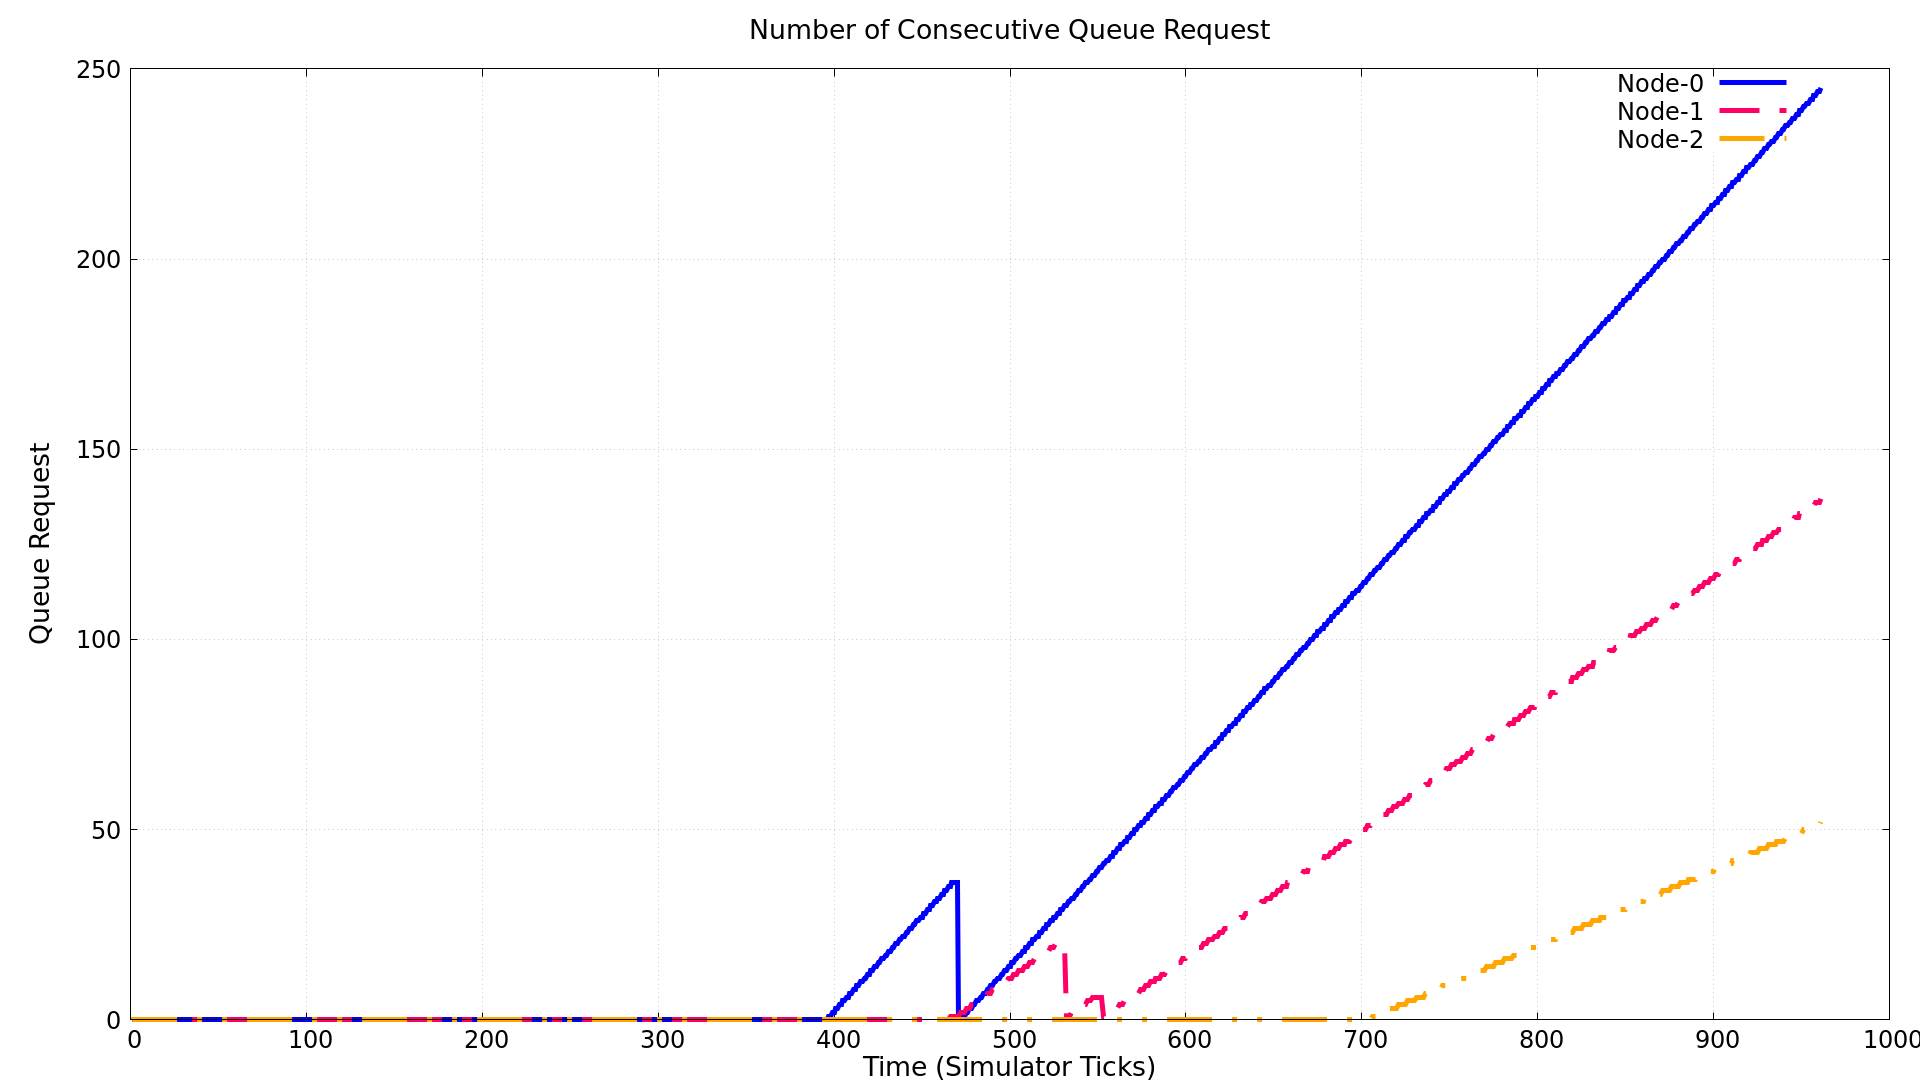
\includegraphics[scale=\plotsize]{plot-request}
	\centering
	\caption{Number of consecutive cycles in which a node has made a request to access a connected node's queue.}
	\label{fig:request}
	\centering
\end{figure}

Due to how the SST model was created, every cycle that a node is idle, it will attempt to request to send a message to another node's queue. This is why for the implemented SST model, the number of consecutive cycles idle is the same as the number of consecutive queue request; see Figure \ref{fig:request} and Figure \ref{fig:idle}.

\begin{figure}[H]
	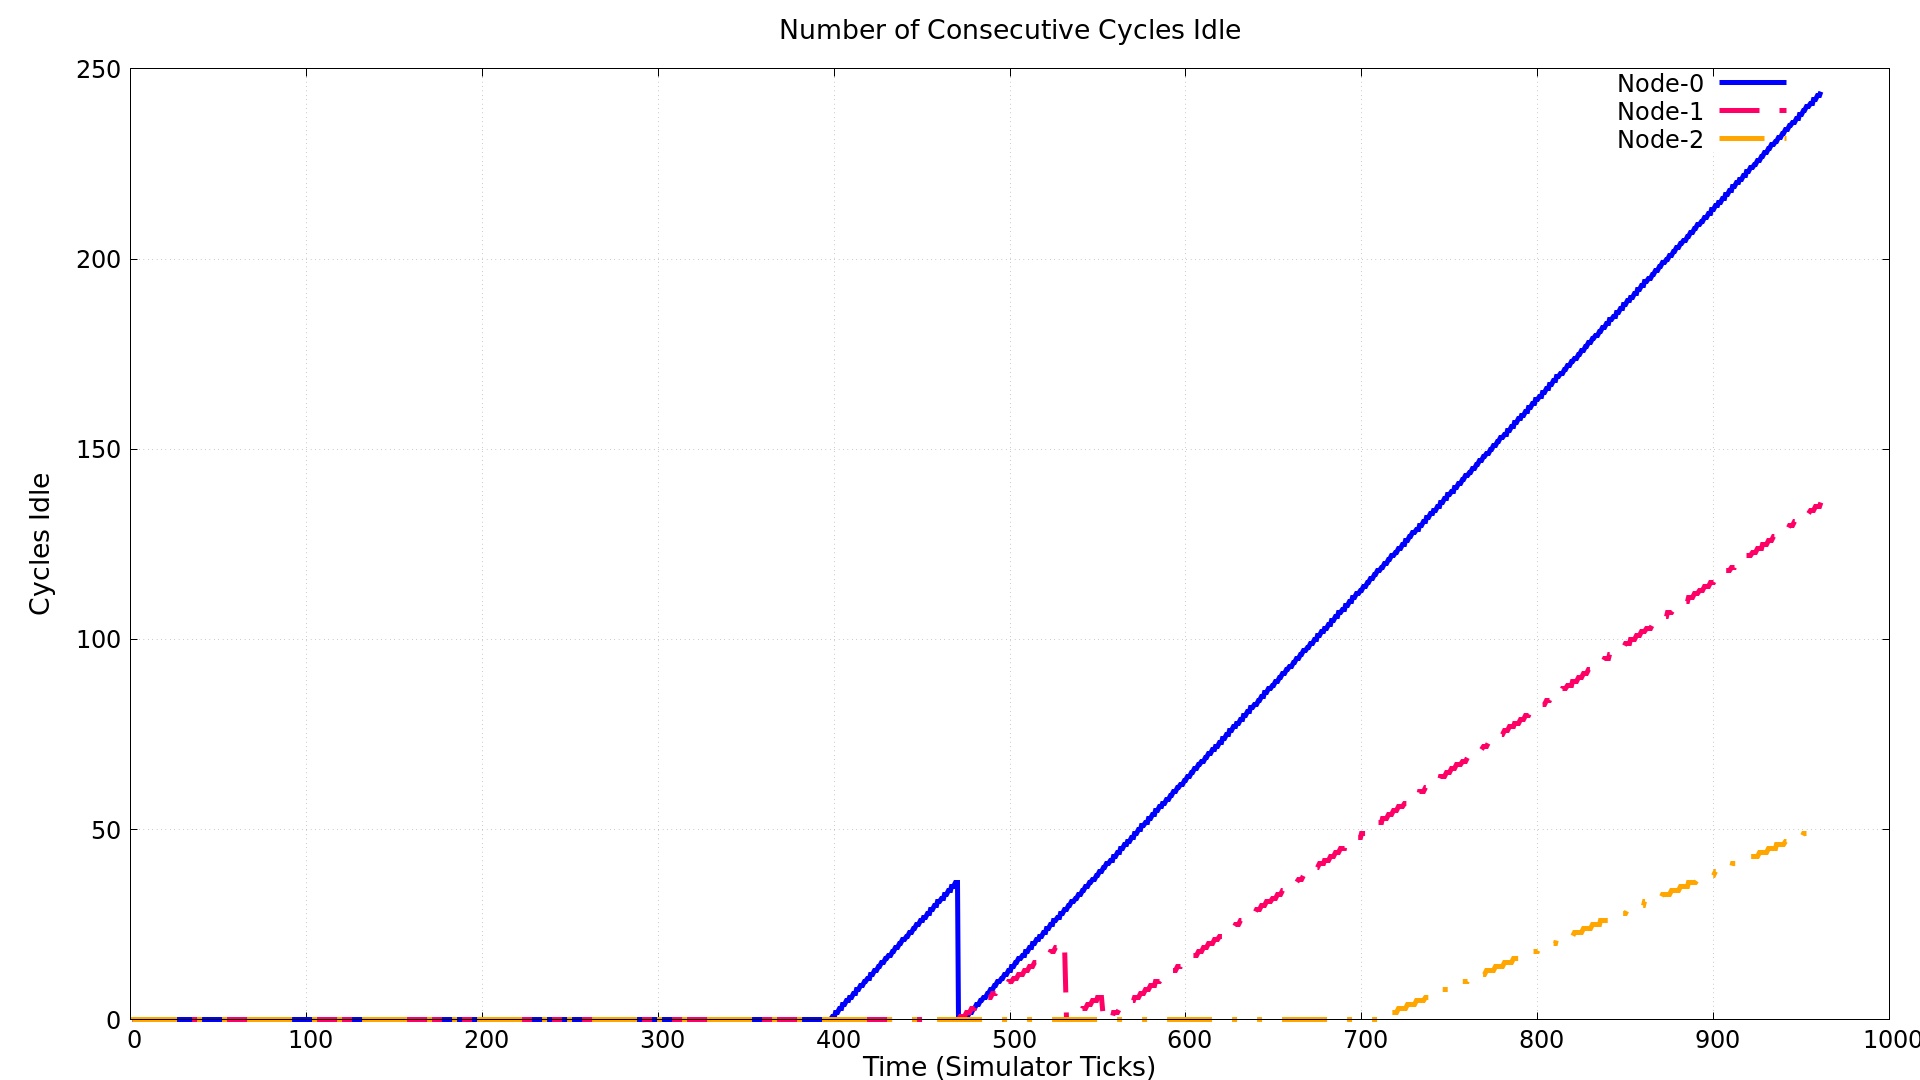
\includegraphics[scale=\plotsize]{plot-idle}
	\centering
	\caption{Number of consecutive cycles in which a node is idle.}
	\label{fig:idle}
	\centering
\end{figure}

At around seven hundred ticks of simulation time, all of the nodes in the simulation stop changing states and remain idle (Figure \ref{fig:state}). The nodes could potentially just be idle; however, all nodes are actively requesting to send messages to a connected nodes queue after seven hundred ticks of simulation time; see Figure \ref{fig:request}. In this case, the system appears to be in a deadlocked state after seven hundred ticks of simulation time.

\begin{figure}[H]
	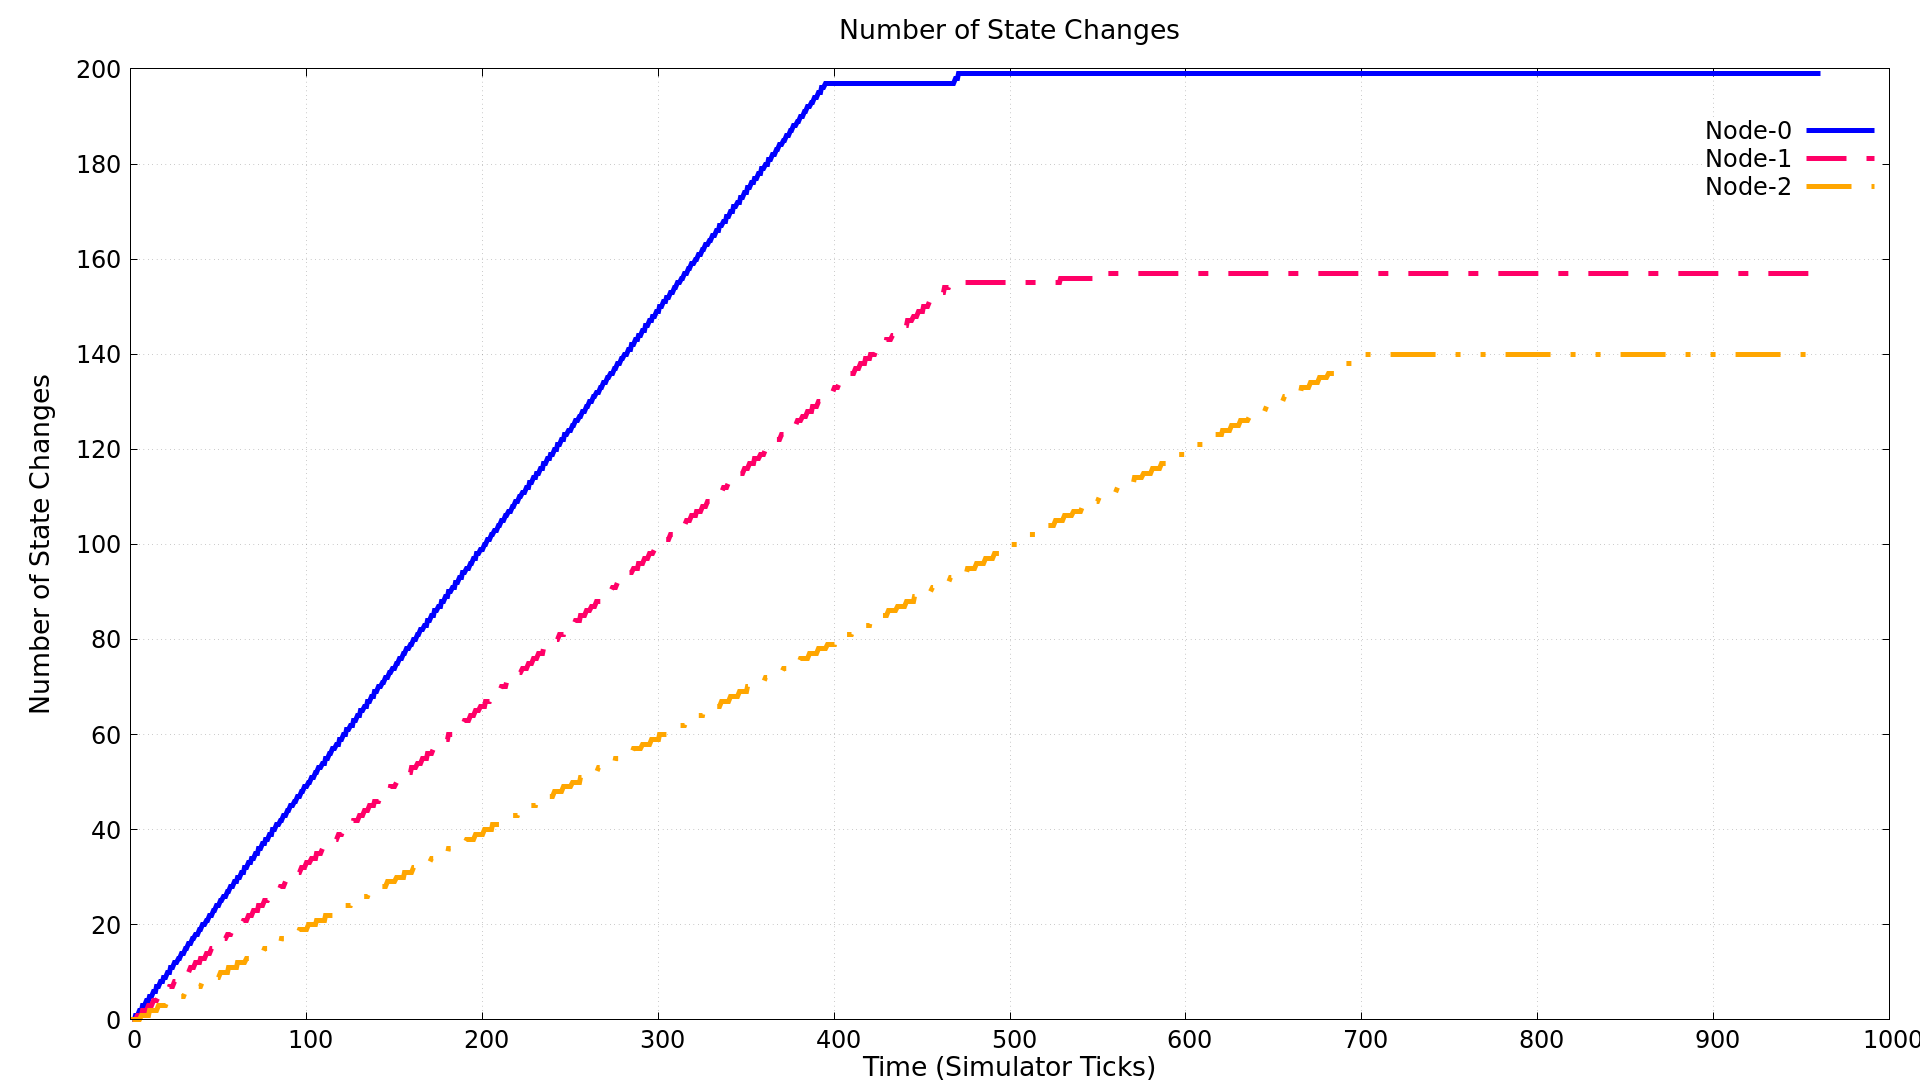
\includegraphics[scale=\plotsize]{plot-state}
	\centering
	\caption{Total number of changes between executing and idle for each node. The longer the value is constant the more likely the node is to be deadlocked.}
	\label{fig:state}
	\centering
\end{figure}

Tracking all three of these metrics is a requirement to declare deadlock in the system. One downside of model two's detection metrics is that it can potentially declare deadlock in a system that is only in transient deadlock. A transient deadlock is a situation where the system could potentially resolve itself out of the deadlocked state over time. In this case, model one might be more useful since it measures all of the nodes' states in a ring and if they are all blocked and idle, then the system is guaranteed to be in a deadlocked state.

For model one, measuring for a circuit of blocked nodes is performed by one node and results in a boolean metric. This metric is only collected during simulation run-time. For model two, the metrics are collected during simulation run-time and stored in variables. The logger node also outputs the data to a file which can be further analyzed later.

% OLD In the first model of the simulation where nodes do not share information with each other, a single node can determine when it is in a blocked state. The node will detect that it has been in a idle state for a predetermined set of time and it has been making request for a node's queue for a large number of time. At this point the node will send out a probe along the ring to determine if other nodes are currently executing. If any nodes are executing, they will drop the probe, otherwise they will pass the probe along. If the sender node receives its own probe, it determines that all nodes are in a deadlocked state so system-deadlock has occurred.

% OLD In the second model of the simulation where nodes share information with a global logging node, edge probing is not required. The logging node can determine when all nodes are in an idle state and have made a large amount of request for a node's queue.


\section{Future Work}
Currently, more work needs to be performed on detecting component-scale deadlock in a simulation. The metrics explained in this report can potentially be used to detect if a ring of nodes is in a deadlocked state, and any nodes outside of the ring - those that must communicate with it - could become deadlocked as well.

The first model will detect deadlock but the second model could detect a transient deadlock if the user defines the thresholds for detection as too small. A combination of both models' detection methods can be used if logger nodes are necessary in the simulation.

The models should be expanded to support more than just a ring topology. The metrics should be tested against these other topologies to see if they still remain accurate.

Finally, the model should support enabling and disabling the conditions for deadlock in different components of the model. The two models explained in this report have the conditions for deadlock baked into the model to force deadlock to occur. Different metrics for deadlock detection could be discovered by making the conditions for deadlock variable.

\bibliographystyle{plain}
\bibliography{biblio}

\end{document}
